\chapter{Classical Algebraic Geometry} \label{classical}

First Chapter stuff

\section{First Section Title}

And now the math begins\dots

\begin{definition}
Given a collection of polynomials $I\subseteq k[x_{1},..., x_{n}]$, the \textbf{affine variety} determined by $I$ is the set
\[
\mathbf{V}(I)=\left\{\mathbf{a}\in k^n\,|\,f(\mathbf{a})=0\text{ for all }f\in I\right\}\subseteq k^n.
\]
This set is sometimes also called the {\bfseries vanishing locus} or {\bfseries zero locus} of $I$. If $I=\lbrace f_{1},..., f_{n}\rbrace$ is a finite collection of polynomials, we we write simply $\mathbf{V}(f_{1},..., f_{n})$.
\end{definition}

\begin{example}
The standard real plane parabola is the affine variety $\mathbf{V}(y-x^{2})$ in ${\bf R}^2$:
\begin{figure}[ht]
    \centering
    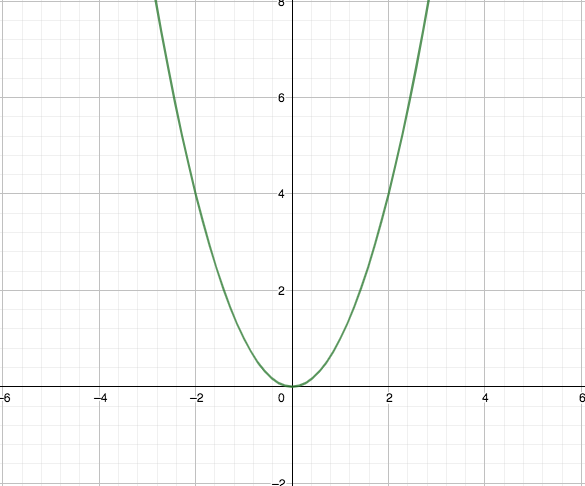
\includegraphics[scale=.25]{Parabolavariety.png}
    %\caption{$y-x^{2}=0$}
\end{figure}
\end{example}


\subsection{Relevant subsection title}

